\documentclass[presentation]{beamer}
\usepackage{common}
\usepackage{arydshln}

\newcommand{\cscat}[1]{$\langle\text{{\itshape#1}}\rangle$}
\newcommand{\csopt}[1]{{\itshape[}#1{\itshape]}}
\newcommand{\csalt}[1]{{\itshape(#1)}}
\newcommand{\op}[1]{\alert{`\texttt{#1}'}}
\newcommand{\operand}[1][\ldots]{{\normalcolor#1}}
\newcommand{\literal}[1]{\texttt{\alert{#1}}}
\newcommand{\bs}{$\backslash$}
\newcommand{\codepath}[1]{../../code/lecture-08/#1}

\AtBeginSubsection[]
{
  \begin{frame}<beamer>
    \frametitle{Next In Line\ldots}
    \tableofcontents[currentsection,currentsubsection]
  \end{frame}
}

\title[\lecturecode{08}]{08 \\ Advanced Aspects of \dotnet}

\author[Giovanni Ciatto]{Giovanni Ciatto\\\texttt{giovanni.ciatto@unibo.it}}

\begin{document}

\frame[label=coverpage]{\titlepage}

\section{Stuctures}

\begin{frame}[allowframebreaks]{Structures as Custom Value Types}
  \begin{block}{Why structures}
    \begin{itemize}
      \item Differently from most platforms, \dotnet let developers define \alert{custom} values types
      \item It does so via the notion of \alert{structures}
      \item Built-in value types (e.g. \texttt{Int32}, \texttt{Boolean}, etc) are defined as structures
    \end{itemize}
  \end{block}

  \begin{block}{Structures vs. Classes}
    Think about structures as ordinary classes, except that:
    %
    \begin{itemize}
      \item they \alert{do not} support \alert{inheritance}
      %
      \begin{itemize}
        \item from neither other structures nor classes
      \end{itemize}

      \item they \alert{can} just implement \alert{interfaces}
      \item their instances are allocated \alert{on the stack}, by default
      \item their instances are passed \alert{by value} through method calls
    \end{itemize}
  \end{block}

  \begin{alertblock}{Purpose of Structures}\centering\itshape
    Defining \alert{lightweight} types whose (de)allocation is \alert{quick}
  \end{alertblock}

  \begin{block}{Syntax of Structures}
    \begin{center}\ttfamily
      struct \cscat{Name} \csopt{: \cscat{Interface Name}} \{ \cscat{Members} \}
    \end{center}
    %
    \begin{itemize}
      \item where \texttt{\cscat{Members}} is an ordinary list of 
      %
      \begin{itemize}
        \item fields, methods, constructors, or properties\ldots
        \item \ldots either static or not\ldots
        \item \ldots similarly to class definitions
      \end{itemize}
      %
    \end{itemize}
  \end{block}

  \begin{alertblock}{Structures are sub-types of \texttt{Object}! (pt. 1)}
    \begin{itemize}
      \item[!] keep in mind to \alert{override} \texttt{Equals}, \texttt{GetHashCode}, and \texttt{ToString} 
    \end{itemize}
  \end{alertblock}

  \tcodeview{1}{6}{25}{\tiny}{\codepath{Structures/Program.cs}}{Example of structure for fractions (a.k.a. rational numbers)}
  \codeview{3}{50}{53}{\tiny}{\codepath{Structures/Program.cs}}

\end{frame}

\subsection{Allocation on the Stack}

\begin{frame}[allowframebreaks]{Reference vs. Value types Allocation}
  \begin{alertblock}{Take away}
    \begin{itemize}
      \item \alert{Reference}-type (i.e. \alert{classes}) objects are allocated on the \alert{heap}
      \item \alert{Value}-type (i.e. \alert{structures}) objects are allocated on the \alert{stack}
      %
      \begin{itemize}
        \item this is what makes them \alert{quick}, provided that the are \alert{small in size}
      \end{itemize}
      \item[!] Such difference brings subtle intricacies in the way reference/value are managed
    \end{itemize}
  \end{alertblock}

  \framebreak

  Consider for instance the \texttt{IPoint} interface, which can either 
  %
  \begin{itemize}
    \item be implemented by the \texttt{CPoint} class
    \item or be implemented by the \texttt{SPoint} class
  \end{itemize}  
  %
  \codeview{1}{26}{44}{\tiny}{\codepath{Structures/Program.cs}}

  \framebreak

  Their instances behave differently, due to the way they are allocated:
  %
  \codeview{3}{55}{67}{\tiny}{\codepath{Structures/Program.cs}}

  \framebreak

  \centering

  \tcodeview{3}{55}{55}{\tiny}{\codepath{Structures/Program.cs}}{Explanation:}
  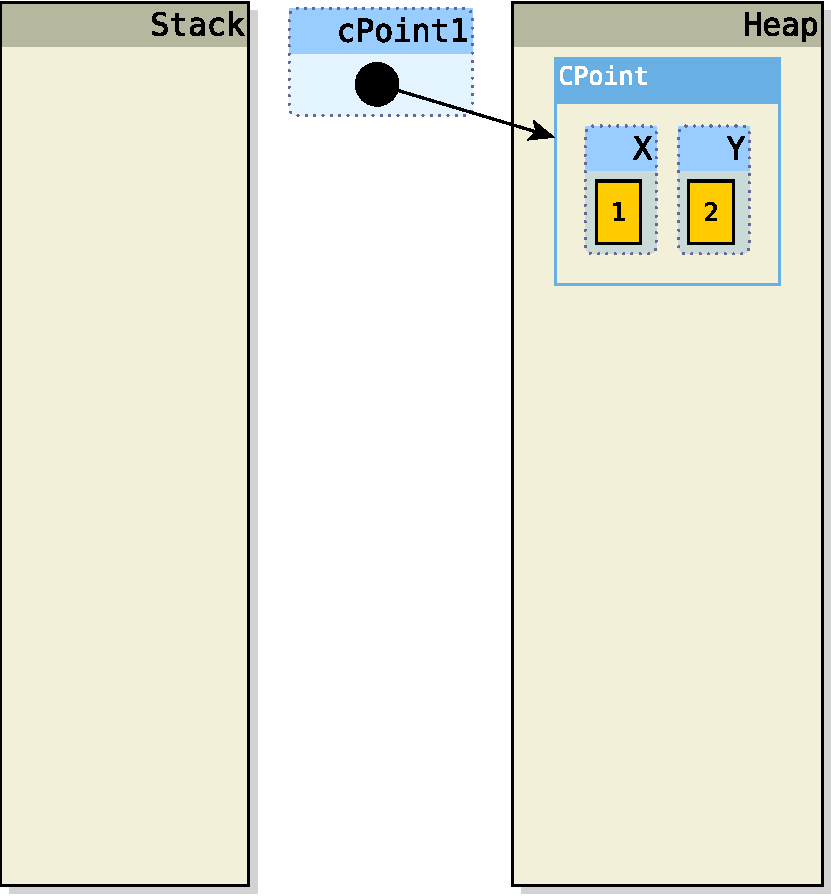
\includegraphics[width=0.4\linewidth]{img/ref-vs-val-anim-1.pdf}

  \framebreak

  \tcodeview{3}{56}{56}{\tiny}{\codepath{Structures/Program.cs}}{Explanation:}
  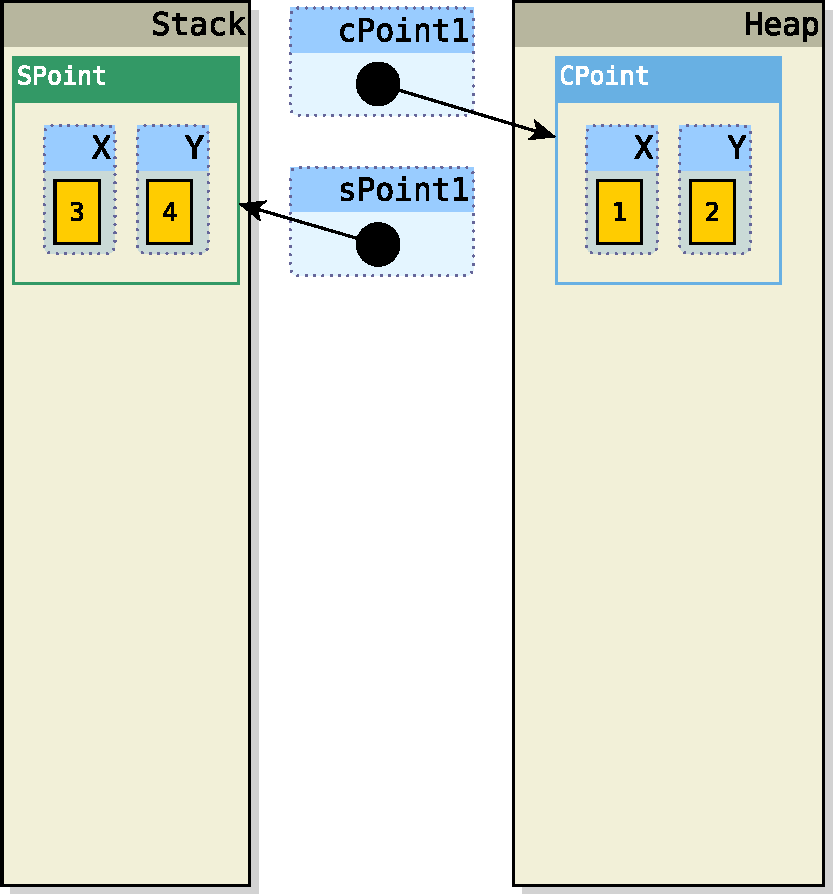
\includegraphics[width=0.4\linewidth]{img/ref-vs-val-anim-2.pdf}

  \framebreak

  \tcodeview{3}{58}{58}{\tiny}{\codepath{Structures/Program.cs}}{Explanation:}
  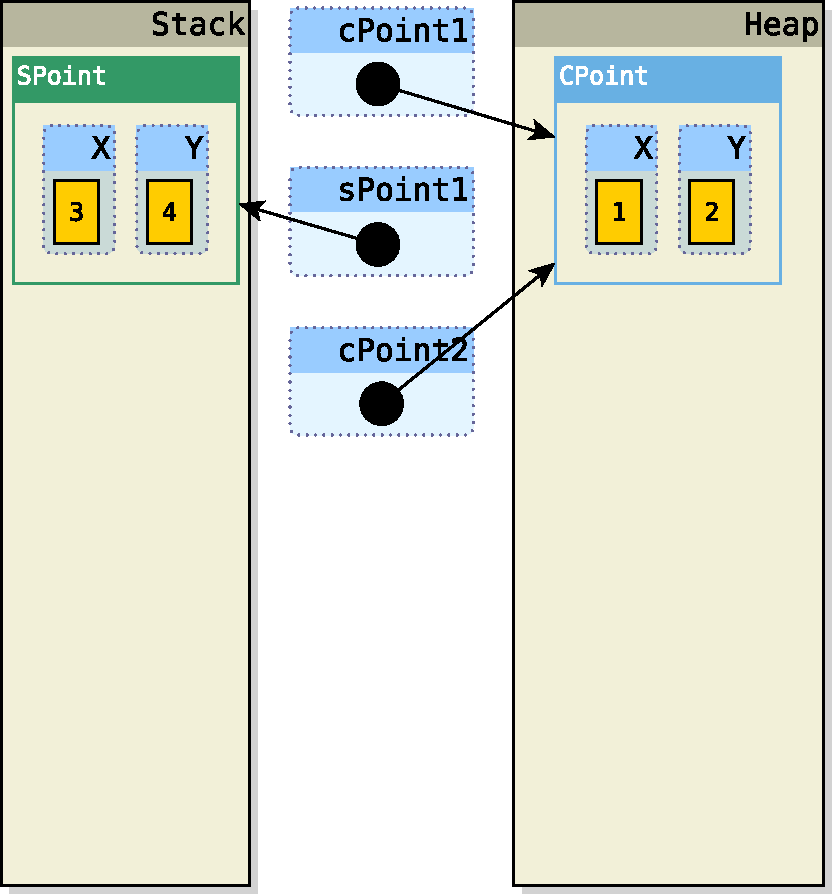
\includegraphics[width=0.4\linewidth]{img/ref-vs-val-anim-3.pdf}

  \framebreak

  \tcodeview{3}{59}{59}{\tiny}{\codepath{Structures/Program.cs}}{Explanation:}
  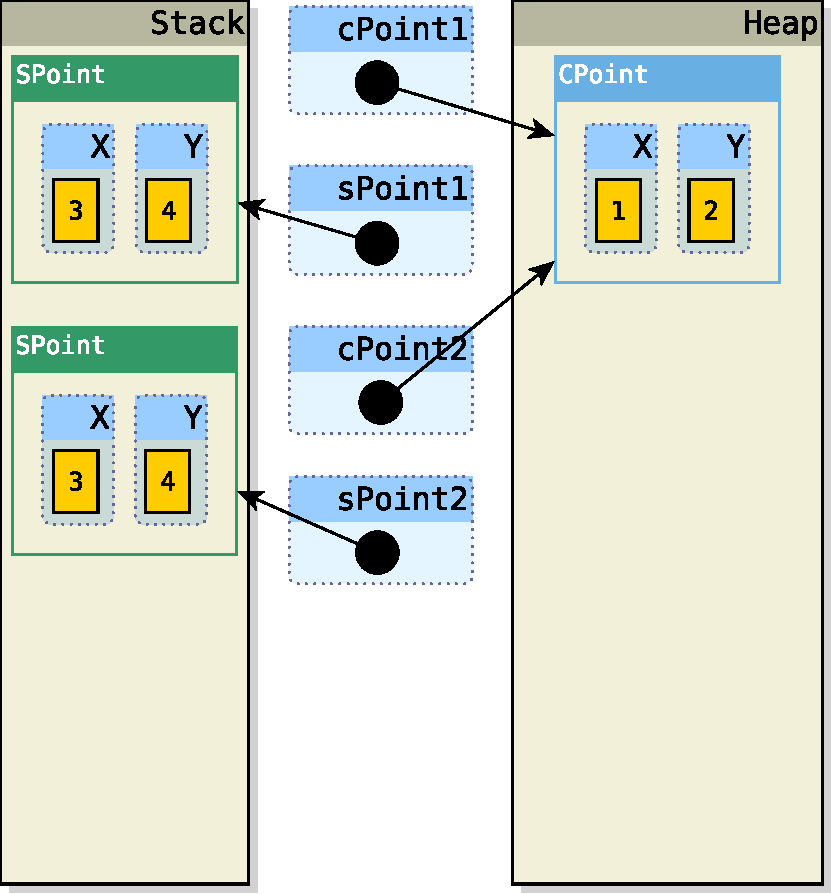
\includegraphics[width=0.4\linewidth]{img/ref-vs-val-anim-4.pdf}

  \framebreak

  \tcodeview{3}{61}{61}{\tiny}{\codepath{Structures/Program.cs}}{Explanation:}
  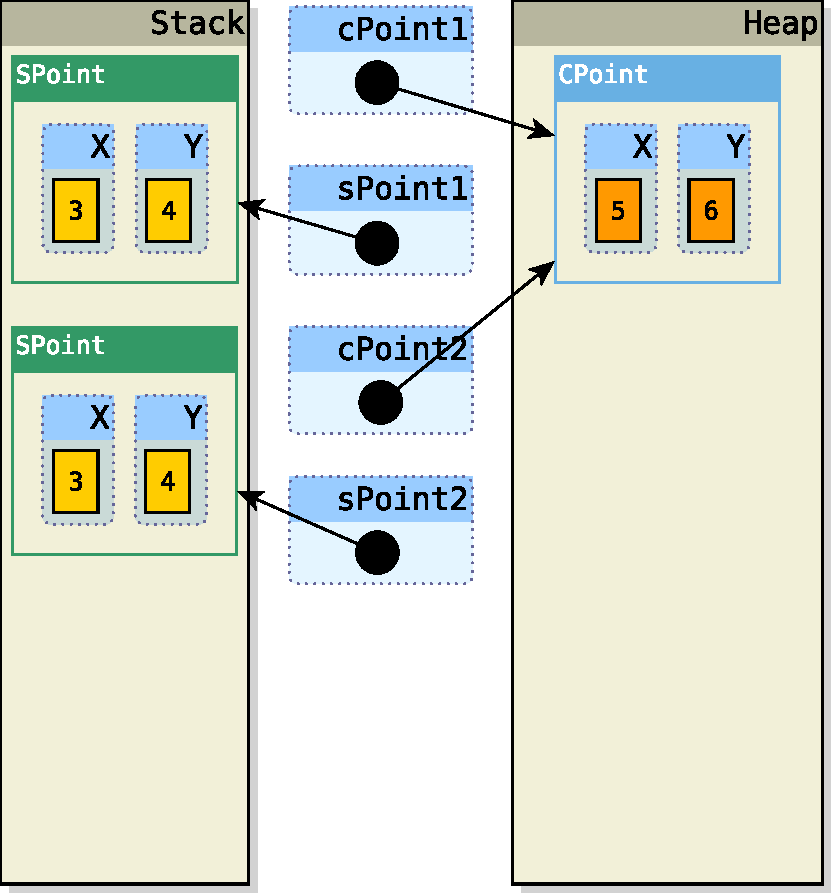
\includegraphics[width=0.4\linewidth]{img/ref-vs-val-anim-5.pdf}

  \framebreak

  \tcodeview{3}{62}{62}{\tiny}{\codepath{Structures/Program.cs}}{Explanation:}
  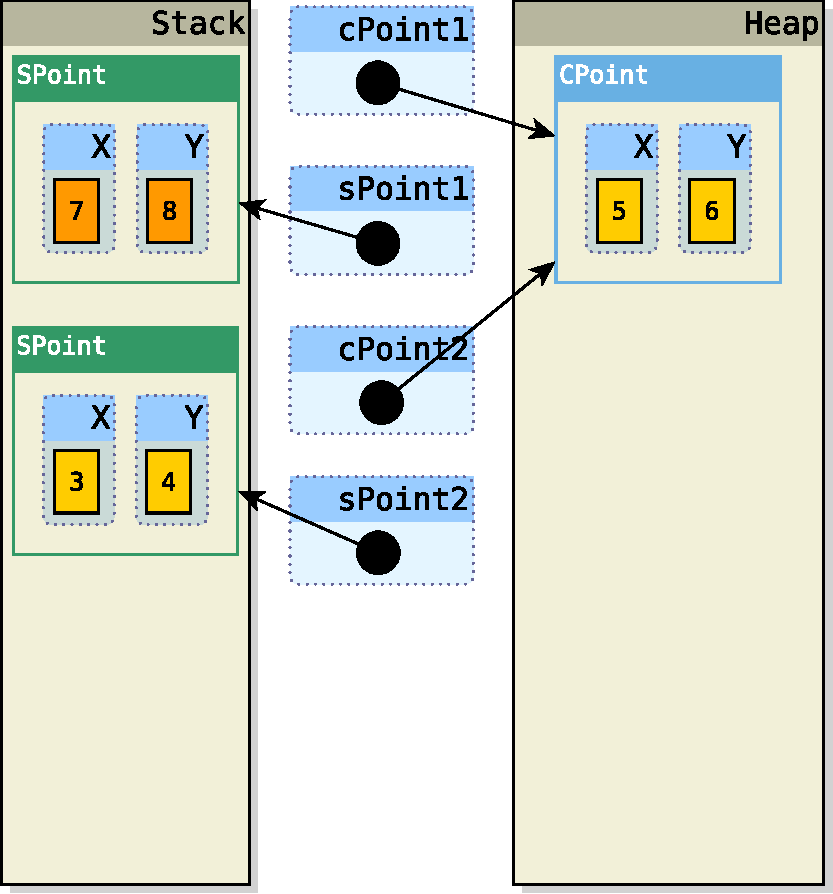
\includegraphics[width=0.4\linewidth]{img/ref-vs-val-anim-6.pdf}

\end{frame}

\subsection{Boxing / Unboxing}

\begin{frame}[allowframebreaks]{Value Types -- Boxing \& Unboxing}
  \begin{block}{Problem}
    \begin{itemize}
      \item All structures are value types
      \item All structures are syb-types of \texttt{Object}, and, possibly, of some interface
      \item \texttt{Object} is a reference type, as well as all interfaces
      \item How can the Liskov substitution principle hold?
    \end{itemize}
  \end{block}

  \begin{exampleblock}{Boxing and unboxing}
    \begin{description}
      \item[Boxing:] $\text{value type} \xrightarrow{assign} \text{reference type}$
      %
      \begin{itemize}
        \item when a value-type object is \alert{assigned} to a reference-type variable, the object is \alert{copied to the heap}
      \end{itemize} 
      \item[Unboxing:] $\text{reference type} \xrightarrow{cast} \text{value type}$
      %
      \begin{itemize}
        \item when a value-type object is \alert{assigned} to a reference-type variable, the object is \alert{copied to the heap}
      \end{itemize}  
    \end{description}
  \end{exampleblock}

  \begin{alertblock}{Keep in mind}
    \begin{itemize}
      \item Boxing and unboxing are \alert{slow} and should be minimised
      \item While unboxing is commonly explicit, boxing is often implicit
      %
      \begin{itemize}
        \item pay attention to the code you write to avoid unexpected boxing
      \end{itemize}
    \end{itemize}
  \end{alertblock}

  \framebreak

  Consider again the \texttt{CPoint}-\texttt{SPoint} example:
  %
  \codeview{3}{55}{62}{\tiny}{\codepath{Structures/Program.cs}}
  %
  consider now the following additional code:
  %
  \codeview{3}{69}{78}{\tiny}{\codepath{Structures/Program.cs}}

  \framebreak

  \begin{center}

  \tcodeview{3}{69}{69}{\tiny}{\codepath{Structures/Program.cs}}{Explanation:}
  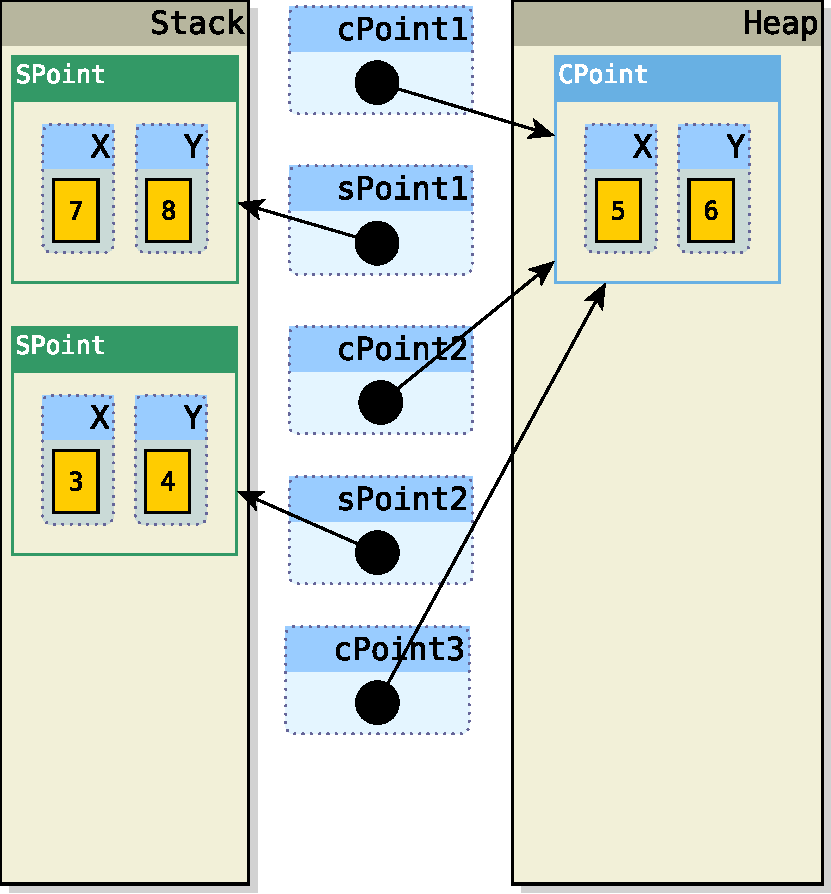
\includegraphics[width=0.4\linewidth]{img/ref-vs-val-anim-7.pdf}

  \framebreak

  \tcodeview{3}{70}{70}{\tiny}{\codepath{Structures/Program.cs}}{Explanation:}
  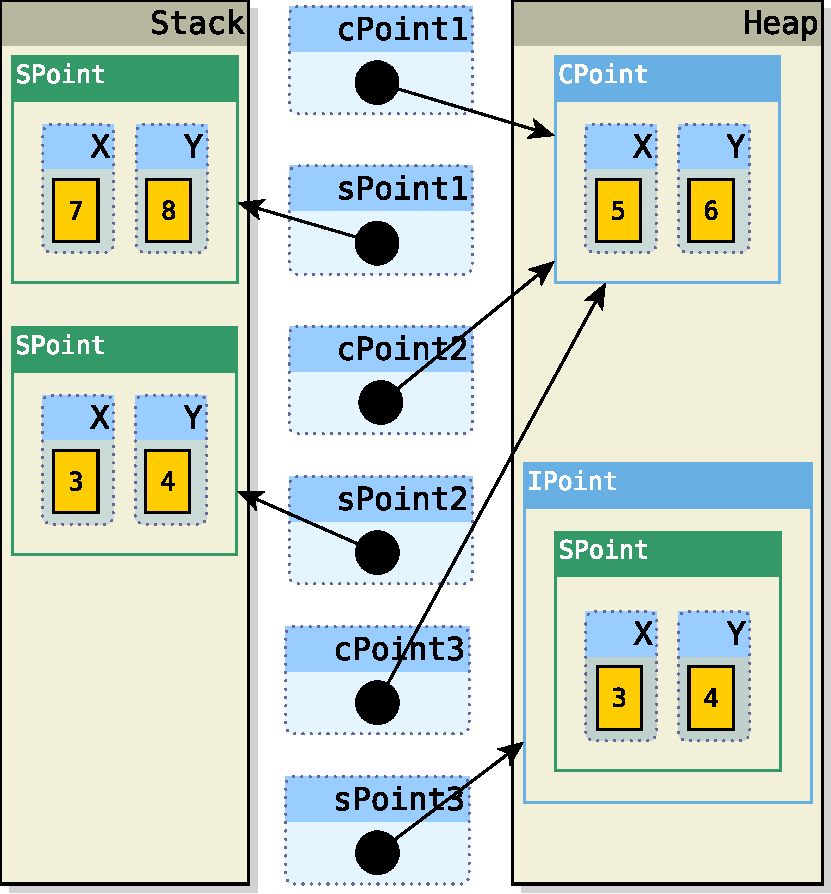
\includegraphics[width=0.4\linewidth]{img/ref-vs-val-anim-8.pdf}

  \framebreak

  \tcodeview{3}{70}{70}{\tiny}{\codepath{Structures/Program.cs}}{Explanation:}
  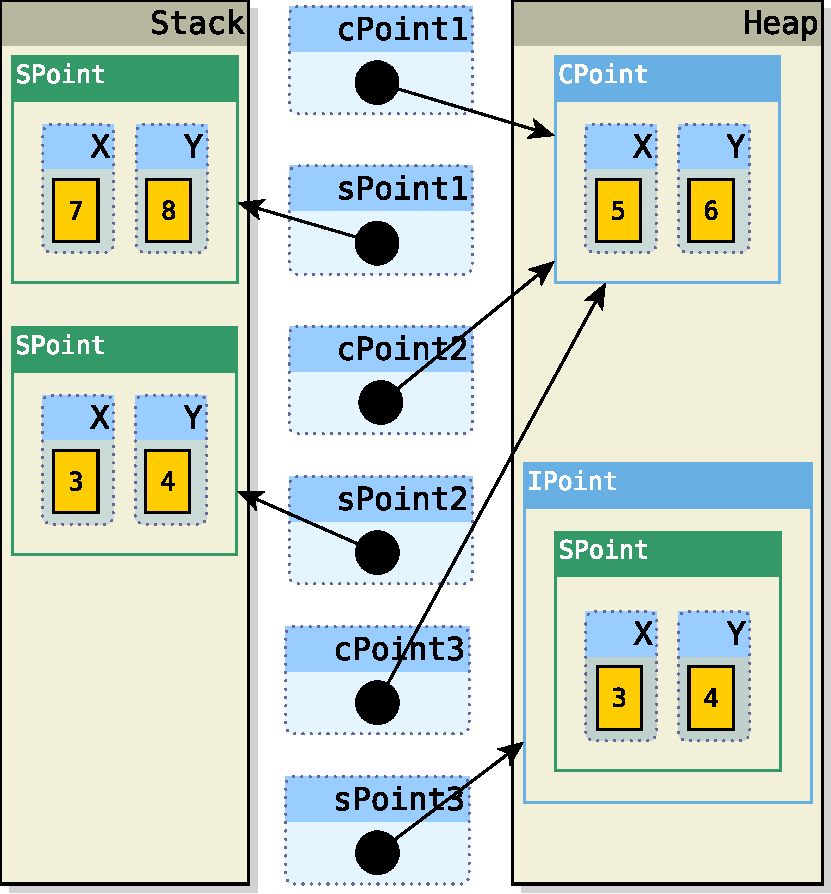
\includegraphics[width=0.4\linewidth]{img/ref-vs-val-anim-8.pdf}

  \framebreak

  \tcodeview{3}{72}{72}{\tiny}{\codepath{Structures/Program.cs}}{Explanation:}
  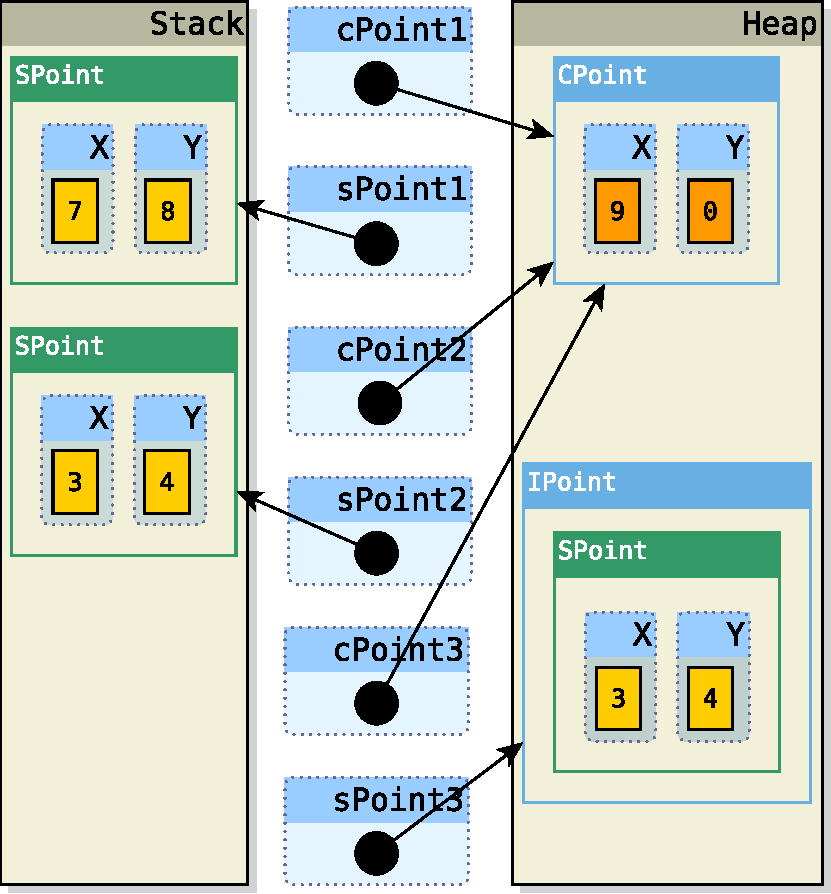
\includegraphics[width=0.4\linewidth]{img/ref-vs-val-anim-9.pdf}

  \framebreak

  \tcodeview{3}{73}{73}{\tiny}{\codepath{Structures/Program.cs}}{Explanation:}
  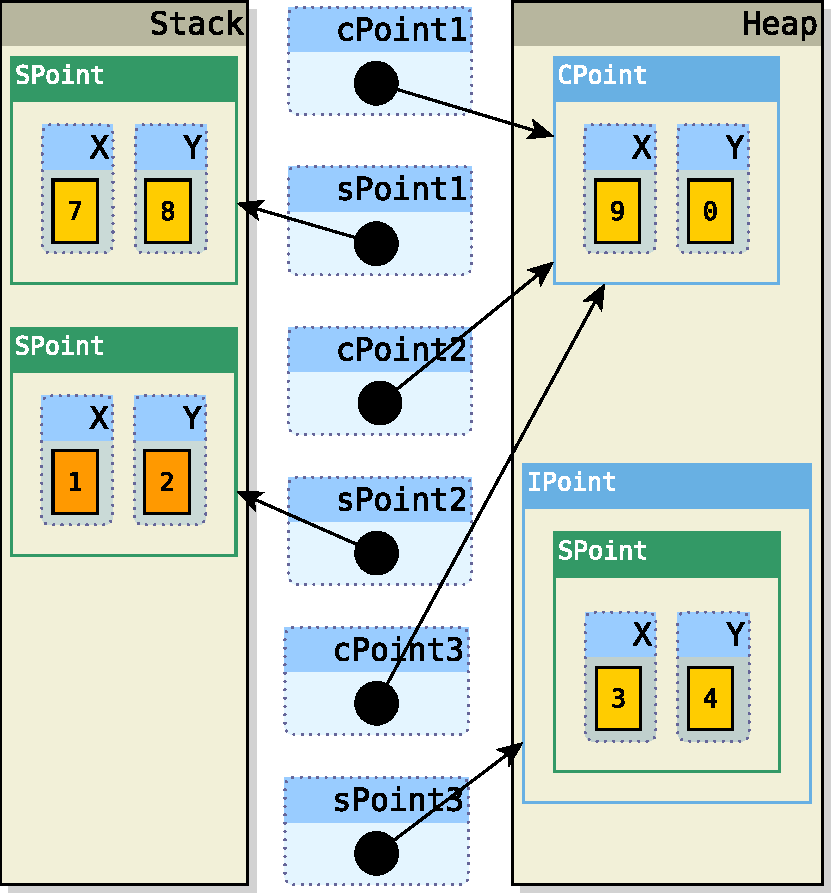
\includegraphics[width=0.4\linewidth]{img/ref-vs-val-anim-10.pdf}

  \end{center}

  \framebreak

  Unboxing is somewhat dual, despite it requires explicit cast:
  %
  \codeview{3}{80}{89}{\tiny}{\codepath{Structures/Program.cs}}

  \framebreak

  \begin{center}

    \tcodeview{3}{80}{80}{\tiny}{\codepath{Structures/Program.cs}}{Explanation:}
    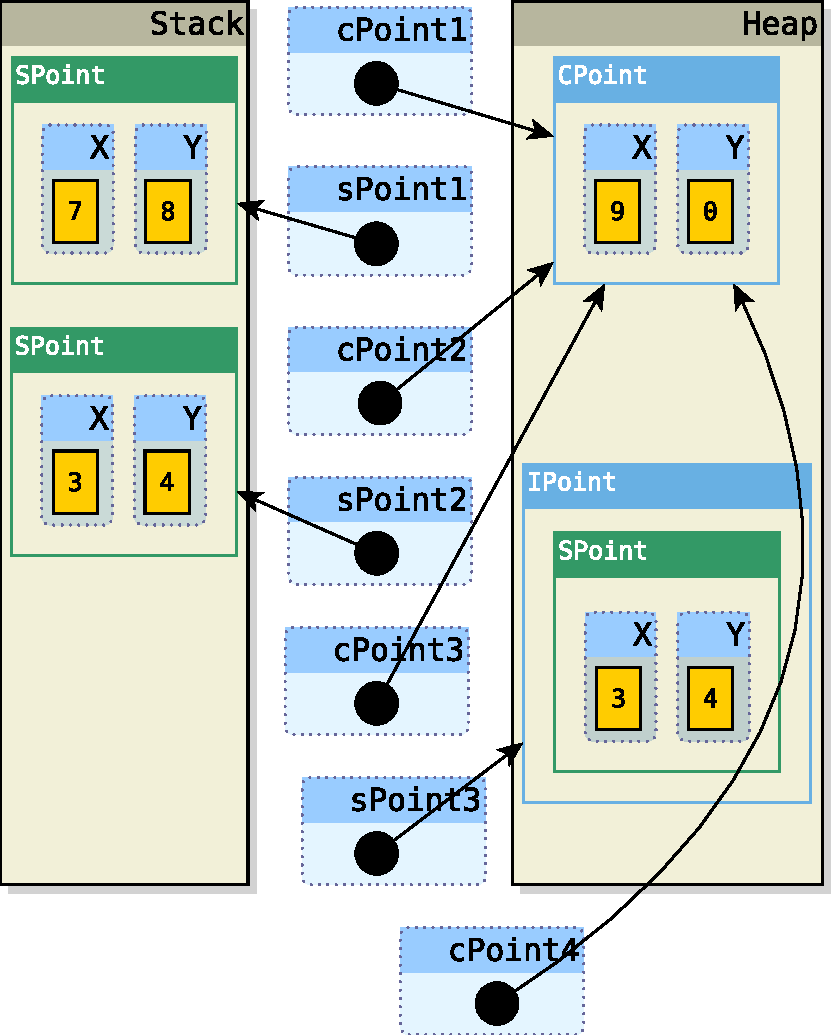
\includegraphics[width=0.4\linewidth]{img/ref-vs-val-anim-11.pdf}
  
    \framebreak
  
    \tcodeview{3}{81}{81}{\tiny}{\codepath{Structures/Program.cs}}{Explanation:}
    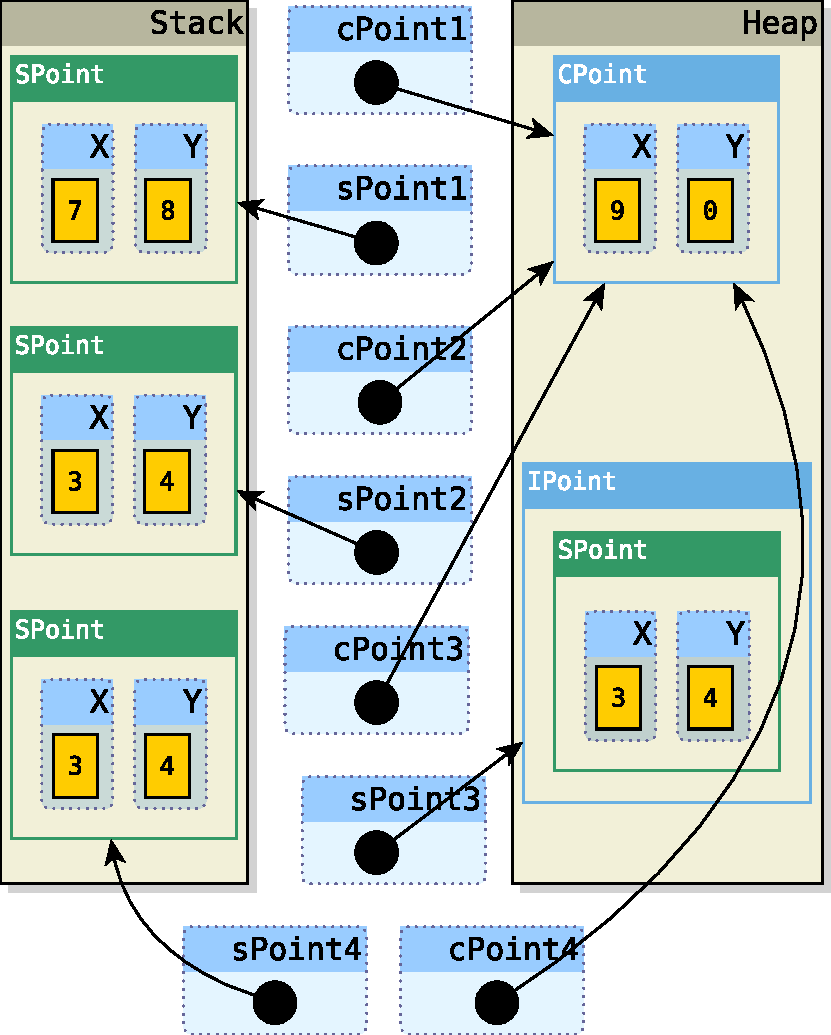
\includegraphics[width=0.4\linewidth]{img/ref-vs-val-anim-12.pdf}
  
    \framebreak
  
    \tcodeview{3}{83}{83}{\tiny}{\codepath{Structures/Program.cs}}{Explanation:}
    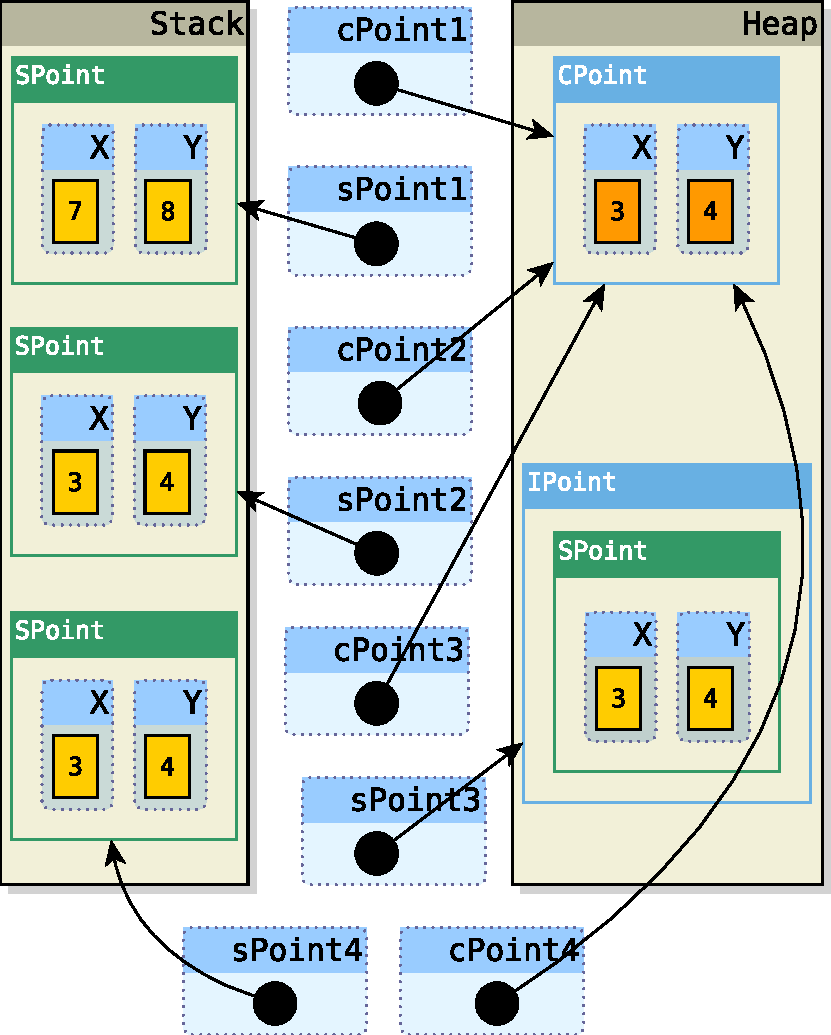
\includegraphics[width=0.4\linewidth]{img/ref-vs-val-anim-13.pdf}
  
    \framebreak
  
    \tcodeview{3}{84}{84}{\tiny}{\codepath{Structures/Program.cs}}{Explanation:}
    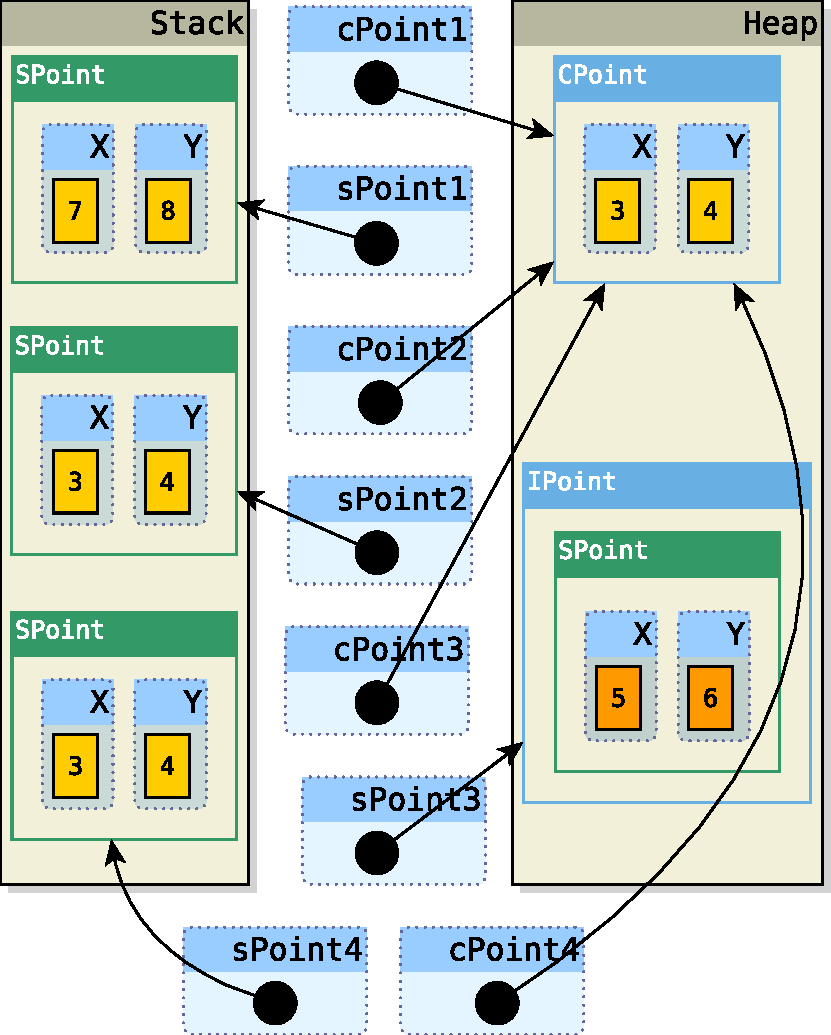
\includegraphics[width=0.4\linewidth]{img/ref-vs-val-anim-14.pdf}
  
    \end{center}

\end{frame}

\section{Method Calls and Parameters}

\begin{frame}{Overview}
  \begin{itemize}
    \item Parameters are \alert{passed} among method calls in different ways
  
    \vfill

    \item Reference (resp. value) types are passed by-reference (resp. by value)
    
    \vfill
    
    \item In general, method calls cannot affect outer variables
    %
    \begin{itemize}
      \item[!] they can alter objects referred by such variables, not their references
      %
      \begin{itemize}
        \item[ie] they can only provoke \alert{side effects}
      \end{itemize}  
    \end{itemize}

    \vfill

    \item Parameters marked as either \texttt{ref} or \texttt{out} can affect outer scopes
    %
    \begin{itemize}
      \item[ie] they can \alert{change} what outer variables are referencing
    \end{itemize}  

    \vfill

    \item Parameters marked as \texttt{params} can occurr 0, 1, or more times
    %
    \begin{itemize}
      \item these are commonly called ``varargs'' in other languages
      \item[$\rightarrow$] such a mechanism lets a method accept a variable amount of arguments
    \end{itemize}

    \vfill

    \item Parameters marked by \texttt{this} let a static method be called as an instance method
  \end{itemize}
\end{frame}

\subsection{Value Types vs. Reference Types}

\begin{frame}[allowframebreaks]{Method Calls with Value/Reference-Type Parameters}
  \begin{block}{Ordinary Method Calls -- General Rules}
    \begin{itemize}
      \item When value-type object are passed, objects are cloned
      \item When reference-type object are passed, only references are cloned
      \item Altering parameters in methods bodies does not affect outer variables
      \item The use case is to support C-like input-output parameters
    \end{itemize}
  \end{block}

  \framebreak

  Consider for instance the following methods:
  %
  \codeview{2}{21}{29}{\tiny}{\codepath{Parameters/Program.cs}}

  \framebreak

  \codeview{3}{43}{63}{\tiny}{\codepath{Parameters/Program.cs}}
  %
  \begin{itemize}\scriptsize
    \item method \texttt{Inc(SomeValueType)} is useless, since it always alters a local copy of \texttt{SomeValueType}
    \item method \texttt{Inc(SomeReferenceType)} works as expected
    \item both methods \texttt{Replace} are meaningless, as the modification they perform on their arguments are not propagated outside 
  \end{itemize}

\end{frame}

\subsection{Ref and Out Parameters}

\begin{frame}[allowframebreaks]{Method Calls with \texttt{ref} Parameters}
  \begin{block}{\texttt{ref} Parameters -- General Rules}
    \begin{itemize}
      \item Formal \texttt{ref} parameters are marked as \texttt{ref} in method signatures
      \item Actual \texttt{ref} parameters are marked as \texttt{ref} in method calls
      \item \texttt{ref} parameters are always passed by reference, even if \texttt{value} types
      \item Re-assigning a \texttt{ref} parameter implies re-assigning some the outer variable which has been passed upon method invocation
    \end{itemize}
  \end{block}

  \framebreak

  Consider for instance the following methods:
  %
  \codeview{2}{31}{39}{\tiny}{\codepath{Parameters/Program.cs}}

  \framebreak

  \codeview{3}{68}{88}{\tiny}{\codepath{Parameters/Program.cs}}
  %
  \begin{itemize}\scriptsize
    \item outer variables are affected by methods manipulations!
  \end{itemize}

\end{frame}

\begin{frame}[allowframebreaks]{Method Calls with \texttt{out} Parameters}
  \begin{block}{\texttt{out} Parameters -- General Rules}
    \begin{itemize}
      \item \texttt{out} parameters are like \texttt{ref} parameters\ldots
      \item \ldots except that they \alert{must} be assigned before before methods return
      %
      \begin{itemize}
        \item otherwise a compilation error is generated
      \end{itemize}
      \item The use case is to support C-like output parameters
    \end{itemize}
  \end{block}

  \framebreak

  Consider for instance the following method:
  %
  \codeview{1}{6}{18}{\tiny}{\codepath{OutputParameters/Program.cs}}
  %
  \begin{itemize}
    \item it attempts to look for the index of an item in an enumerable
    %
    \begin{itemize}
      \item returning \texttt{true} if the item is found
      \item or \texttt{false} otherwise
    \end{itemize}
    \item in case the item is found, its index is stored into the output parameters
  \end{itemize}

  \framebreak

  \tcodeview{3}{24}{33}{\tiny}{\codepath{OutputParameters/Program.cs}}{Usage example:}
  
\end{frame}

\subsection{Varargs}

\begin{frame}[allowframebreaks]{Method Calls with Variable Parameters}
  \begin{block}{\texttt{param} Parameters -- General Rules}
    \begin{itemize}
      \item Parameters marked as \texttt{param} in method signatures\ldots
      
      \item \ldots can be provided in arbitrary amounts upong method calls
      %
      \begin{itemize}
        \item[eg] 0, 1, or more
      \end{itemize}

      \item They are treated as \alert{arrays} within methods
      
      \item They are treated as ordinary arguments outside methods
    
      \item The use case is to support a variable amount of arguments as input
    \end{itemize}
  \end{block}

  \framebreak

  Consider for instance the following method:
  %
  \codeview{1}{7}{16}{\tiny}{\codepath{Varargs/Program.cs}}
  %
  \begin{itemize}
    \item this is a generic method aimed at creating and filling an \texttt{ISet<T>}
    \item it accepts 1 + $N$ parameters of type \texttt{T}
    %
    \begin{itemize}
      \item where $N$ may be 0, 1, or more
    \end{itemize}
    \item it is handy since \texttt{T} is automatically inferred in method calls
    %
    \begin{itemize}
      \item and must not explicitly provided by developers
    \end{itemize}
  \end{itemize}

  \framebreak

  \tcodeview{3}{22}{32}{\tiny}{\codepath{Varargs/Program.cs}}{Usage example:}
  
\end{frame}

\subsection{Extension Methods}

\begin{frame}[allowframebreaks]{Extension Methods}
  \begin{block}{Extension Methods -- General Rules}
    \begin{itemize}
      \item Method defined in non-generic, non-nested static classes can be marked as extensions
      \item The first argument of an extension method is marked by \texttt{this}
      \item Extension methods may work as ordinary static methods\ldots
      \item \ldots but they can also be called as if they were instance methods
      %
      \begin{itemize}
        \item[!] instance methods of the type of the argument marked by \texttt{this}
      \end{itemize}
      \item Their use case is to add functionalities to a pre-existing type
      %
      \begin{itemize}
        \item whose definition cannot or should not be extended/altered
        %
        \begin{itemize}
          \item[eg] interfaces, sealed classes, structures, enums, etc.
        \end{itemize}
        \item without requiring any edit to the type definiton
      \end{itemize}
    \end{itemize}
  \end{block}

  \framebreak

  Consider for instance the following method:
  %
  \codeview{2}{11}{20}{\tiny}{\codepath{ExtensionMethods/Program.cs}}
  %
  \begin{itemize}
    \item it aims at converting a string into \texttt{AlTeRnAtE CaSe}
    \item it exploits a \texttt{StringBuilder}
    %
    \begin{itemize}
      \item[ie] an object aimed at creating a string incrementally
    \end{itemize}
    \item notice the first argument is of type \texttt{string} and it is marked by \texttt{this}
    %
    \begin{itemize}
      \item meaning that this is an extension method, extending the \texttt{string} type
      %
      \begin{itemize}
        \item[$\rightarrow$] the method can be invoked on strings as an instance method:
        %
        \codeview{3}{42}{43}{\tiny}{\codepath{ExtensionMethods/Program.cs}}
      \end{itemize}
    \end{itemize}
  \end{itemize}

  \framebreak

  \begin{alertblock}{Generic Extension Method}
    \begin{itemize}
      \item Common practice: combining extension and generic methods\ldots
      \item \ldots to add functionalities to a wide range of type at once
    \end{itemize}
  \end{alertblock}

  \framebreak

  Consider for instance the following method:
  %
  \codeview{2}{22}{35}{\tiny}{\codepath{ExtensionMethods/Program.cs}}
  %
  \begin{itemize}
    \item it converts any enumerable of any type \texttt{T} into a string
    \item where the items of the enumerable are representes as strings, separated by \texttt{delimiter}
    \item and the whole string is wrapped between \texttt{prefix} and \texttt{suffix}
  \end{itemize}

  \tcodeview{3}{45}{49}{\tiny}{\codepath{ExtensionMethods/Program.cs}}{Usage Example}

  \framebreak

  \begin{alertblock}{Name clashing in Extension Methods}
    \begin{itemize}
      \item Of course an extension method may have the same name of some actual instance method of a type
      \item[!] When this is the case, actual instace methods take priority over extension methods
    \end{itemize}
  \end{alertblock}

  \framebreak

  Consider for instance the following method:
  %
  \codeview{2}{37}{38}{\tiny}{\codepath{ExtensionMethods/Program.cs}}
  %
  \begin{itemize}
    \item it is an extension methods for strings
    \item notice the \texttt{String} class has an instance method named \texttt{ToUpper}
    \item[$\rightarrow$] in case of ambiguity, the original method of \texttt{String} is invoked
  \end{itemize}

  \tcodeview{3}{51}{52}{\tiny}{\codepath{ExtensionMethods/Program.cs}}{One can reveal this rule as follows:}
  %
  \begin{itemize}
    \item $1^{st}$ invocation is ambigous, then the original \texttt{ToUpper} method is called
    \item $2^{nd}$ one is not, then the extension method is invoked
    %
    \begin{itemize}
      \item which provokes an exception!
    \end{itemize}
  \end{itemize}

\end{frame}

\section{Enums}

\begin{frame}[allowframebreaks]{Enums}
  \begin{block}{About enums}
    \begin{itemize}
      \item Enums are fixed-size groups of related constants
      %
      \begin{itemize}
        \item[eg] days of week, months of the year, seasons, gender  
      \end{itemize}

      \item OOP languages usually represents groups of related constants as types
      %
      \begin{itemize}
        \item \ldots having a fixed amount of instances
      \end{itemize}

      \item Such types are called \alert{enum} types, and they have an ad-hoc syntax

      \item In \dotnet{} enums must be sub-types of some built-in integer type
      %
      \begin{itemize}
        \item[ie] \texttt{(U)Int16/32/64}, or \texttt{(S)Byte}
        \item[$\rightarrow$] \dotnet enums are value-types
        \item[$\rightarrow$] \dotnet enums are integers 
      \end{itemize}
    \end{itemize}
  \end{block}

  \begin{block}{Syntax}
    \begin{center}\ttfamily
      enum \cscat{Name} \csopt{: \cscat{Integer Type}} \{ \cscat{Constants} \}
    \end{center}
    %
    \begin{itemize}
      \item where \texttt{\cscat{Name}} is the name of the enum type being defined
      \item and \texttt{\cscat{Integer Type}} is one of \texttt{(U)Int16/32/64}, or \texttt{(S)Byte}
      %
      \begin{itemize}
        \item defaults to \texttt{Int32} in case it is missing
      \end{itemize}
      \item and \cscat{Constants} is a number of comma-separated symbols in \texttt{PascalCase}
      %
      \begin{itemize}
        \item optionally assigned to their values
      \end{itemize}
    \end{itemize}
  \end{block}

  \tcodeview{1}{5}{14}{\tiny}{\codepath{Enums/Program.cs}}{Example of \texttt{enum}}
  \tcodeview{3}{51}{57}{\tiny}{\codepath{Enums/Program.cs}}{Usage of \texttt{enum}}
  %
  \begin{itemize}
    \item notice enums are essentially integers
  \end{itemize}
\end{frame}

\begin{frame}[allowframebreaks]{Flag Enums}
  \begin{block}{Common practice: flag enums}
    \begin{itemize}
      \item If an enum values are less than 64\ldots
      \item \ldots and you may need to group enum values together
      \item then you may consider implementing you enum as a \alert{flag}
      \item Flag enums are enums whose values correspond to powers of 2
      %
      \begin{itemize}
        \item bitwise operators can then be exploited to speed-up or simplify some tasks
      \end{itemize}
    \end{itemize}
  \end{block}

  \framebreak

  Consider again the \texttt{SingleDayOfWeek}:
  \codeview{1}{5}{14}{\tiny}{\codepath{Enums/Program.cs}}
  %
  \begin{itemize}
    \item this is not a flag enum (values are not powers of 2)
  \end{itemize}

  \framebreak

  Imagine you need a means to determine if a day is:
  %
  \begin{enumerate}\small
    \item part of the weekend or not
    \item even or odd (knowing that Sunday is not considered as even nor as odd)
  \end{enumerate}
  %
  \codeview{2}{37}{41}{\tiny}{\codepath{Enums/Program.cs}}
  %
  \begin{itemize}
    \item these methods must take the indexing of values into account
  \end{itemize}

  \framebreak

  Alternatively, one may model the days of week as a flag enum:
  %
  \codeview{1}{16}{33}{\tiny}{\codepath{Enums/Program.cs}}
  %
  \begin{itemize}
    \item groups of days can be modelled as well
  \end{itemize}

  \begin{exampleblock}{Why do flag enums need power of two?}
    \begin{itemize}
      \item Each position in an integer correspond to the presence/lack of a value
      \item Sets of values can be represented as by integers
    \end{itemize}
    \[
      \begin{array}{rcl}
        \mathtt{Monday} = & 1 & = 0000 0001\\
        \mathtt{Wednesday} = & 4 & = 0000 0100\\
        \mathtt{Friday} = & 16 & = 0001 0000\\
        \hline
        \mathtt{None} = & 0 & = 0000 0000\\
        \mathtt{OddDays} = & 21 & = 0001 0101\\
      \end{array}
    \]
  \end{exampleblock}

  \medskip

  So, the aforementioned methods can be conveniently implemented:
  %
  \codeview{2}{43}{47}{\tiny}{\codepath{Enums/Program.cs}}

\end{frame}

\begin{frame}[allowframebreaks]{The \texttt{Enum} class}
  \begin{block}{About the \texttt{Enum} class}
    \begin{itemize}
      \item It is the super-type of all enums
      \item It comes with a number of useful static methods aimed at:
      %
      \begin{itemize}
        \item Enumerate the values of a given enum
        \item Parse the values of a given enum from string
        \item Get the names of the values of a given array
      \end{itemize}

      \item cf. \url{https://docs.microsoft.com/dotnet/api/system.enum}
    \end{itemize}
  \end{block}

  \framebreak

  \tcodeview{3}{59}{64}{\tiny}{\codepath{Enums/Program.cs}}{Example 1 -- Enumerating values and getting names}
  \lstinputlisting[basicstyle=\ttfamily\tiny]{snippets/output1.txt}

  \framebreak

  \tcodeview{3}{66}{72}{\tiny}{\codepath{Enums/Program.cs}}{Example 2 -- Parsing values}
  \lstinputlisting[basicstyle=\ttfamily\tiny]{snippets/output2.txt}
\end{frame}

\section{Events and Listners}

\begin{frame}[allowframebreaks]{The Observer Pattern}
  Observer pattern\footnote{cf. \url{https://en.wikipedia.org/wiki/Observer_pattern}} (a.k.a. event-listener, a.k.a. publish-subscribe):
  %
  \begin{itemize}
    \item lets an entity \alert{react} to relevant events concerning another entity

    \item two entities involved: 
    %
    \begin{description}
      \item[subject] is the entity whose events are of interest
      %
      \begin{itemize}
        \item[aka] obervable,  publisher, or event source
      \end{itemize} 

      \item[observer] is the entity willing to react to events
      %
      \begin{itemize}
        \item[aka] listener, or subscriber
      \end{itemize} 
    \end{description}

    \item involves two phases:
    %
    \begin{enumerate}
      \item the observer registers its interest to the subject
      \item the subject notifies all the registered observers whenever an event occurs
    \end{enumerate}

    \framebreak

    \item in OOP, event notification are commonly reified into method calls

    \item when reified into OOP code, the subject needs 3 methods
    %
    \begin{enumerate}
      \item a method to let subjects register
      \item a method to let subjects unregister
      \item a (possibly private) method to propagate events to observers
    \end{enumerate}

    \item when reified into OOP code, the observer needs 1 method
    %
    \begin{itemize}
      \item specifying what to do whenever a new event notifaction is 
    \end{itemize}

    \item in a nutshell:
    %
    \begin{center}
      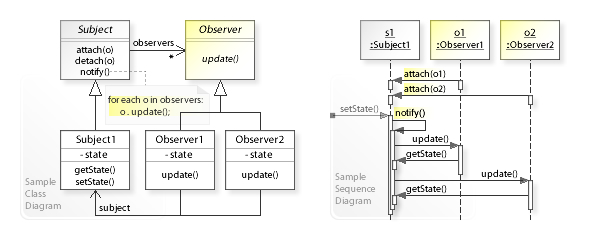
\includegraphics[width=.8\linewidth]{img/observer-pattern.jpg}
    \end{center}

  \end{itemize}
\end{frame}

\begin{frame}[allowframebreaks]{\dotnet Events}
  \begin{block}{About \dotnet events}
    \begin{itemize}
      \item \dotnet provides bult-in support to the observer pattern via events
      \item Events are yet another sort of member in \dotnet classes/interfaces
      \item The event source/listener nomenclature is adopted in \dotnet
      \item Classes corresponding to event sources may expose a number of named events
      \item Each event defines the type of the listener which may register to it
      \item Event listeners are instances of some delegate type (i.e. functions)
    \end{itemize}
  \end{block}

  \begin{block}{Syntax -- Definition Side}
    \begin{center}\ttfamily
      event \cscat{Delegate Type} \cscat{Event Name};
    \end{center}
    \begin{itemize}
      \item where \texttt{\cscat{Event Name}} is the name of the event, \texttt{PascalCase}
      \item and \texttt{\cscat{Delegate Type}} is some delegate denoting the possible type of listeners for \texttt{\cscat{Event Name}}
      %
      \begin{itemize}
        \item most commonly \texttt{Action<T>}
      \end{itemize}
    \end{itemize}
  \end{block}

  \begin{block}{Syntax -- Usage Side (Listener Registration)}
    \begin{center}
      \texttt{\cscat{Object}\alert{.}\cscat{Event Name} \alert{+=} \cscat{Event Listener};}
      \\
      or
      \\
      \texttt{\cscat{Object}\alert{.}\cscat{Event Name} \alert{-=} \cscat{Event Listener};}
    \end{center}
    \begin{itemize}
      \item to (un)register an \texttt{\cscat{Event Listener}} for \texttt{\cscat{Event Name}}
      \item assuming \texttt{\cscat{Object}} defines an event named \texttt{\cscat{Event Listener}}
      \item and \texttt{\cscat{Event Listener}} matches the type of \texttt{\cscat{Event Name}}
    \end{itemize}
  \end{block}

  \begin{block}{Syntax -- Usage Side (Event Propagation)}
    \begin{center}
      \texttt{\cscat{Object}.\cscat{Event Name}\alert{?.}Invoke(\cscat{Args});}
      \\
      or
      \\
      \texttt{if (\cscat{Object}.\cscat{Event Name} != null) \{ \cscat{Object}\alert{.}\cscat{Event Name}(\cscat{Args}) \}}
    \end{center}
    \begin{itemize}
      \item where the amounts and types of \texttt{\cscat{Args}} depend on the type of \texttt{\cscat{Event Name}}
    \end{itemize}
  \end{block}

\end{frame}

\begin{frame}[allowframebreaks]{\dotnet Events -- Example}

  \tcodeview{1}{6}{16}{\tiny}{\codepath{Events/Program.cs}}{An interface exposing an event}
  %
  \begin{itemize}
    \item instances of \texttt{IButton} are buttons having a particular purpose
    %
    \begin{itemize}
      \item[eg] the name of the button (Esc, Enter, Tab, etc.)
    \end{itemize}

    \item buttons can be pressed via the \texttt{Press()} method
    
    \item whenver the button is pressed, the \texttt{OnPressed} event is propagated to listeners
    %
    \begin{itemize}
      \item and the purpose of the event is passed to each listener
    \end{itemize}
  \end{itemize}

  \framebreak

  \tcodeview{1}{17}{33}{\tiny}{\codepath{Events/Program.cs}}{A class triggering an event}

  \framebreak

  \tcodeview{2}{37}{52}{\tiny}{\codepath{Events/Program.cs}}{Usage of events}

\end{frame}

\section{Operator Overloading}

\begin{frame}{Inconsistencies in \csharp Operators}
  \begin{block}{Consider the \texttt{==} operator\ldots}
    \begin{itemize}
      \item It compares refernce types by reference (i.e. checks for identity)
      \item It compares strings by value
      %
      \begin{itemize}
        \item[!] notice that strings are reference types!
      \end{itemize}
      \item It compares integers by value
      \item[\vdots] 
    \end{itemize}
  \end{block}

  \begin{block}{Consider the \texttt{+=} operator\ldots}
    \begin{itemize}
      \item It compares increases numbers
      \item It concatenates strings
      \item It adds listeners to events
      \item[\vdots] 
    \end{itemize}
  \end{block}

  \begin{itemize}
    \item[!] How are all such inconsistencies possible?
  \end{itemize}
\end{frame}

\begin{frame}[allowframebreaks]{Operators Overloading}
  \begin{exampleblock}{Definition}\centering
    Operator overloading is a feature letting OOP languages redefine the semantics of some operators on a per-type basis
  \end{exampleblock}

  \begin{block}{In \dotnet}
    \begin{itemize}
      \item \dotnet supports operator overloading on classes, via static methods
      %
      \begin{itemize}
        \item since version 8, operator overloading is supported for interfaces too
      \end{itemize}

      \item only a predefined set of operators can be overloadaded
      %
      \begin{itemize}
        \item[eg] \texttt{+}, \texttt{-}, \texttt{*}, \texttt{/}, \texttt{==}, \texttt{!=}, \texttt{>}, \texttt{<}, etc
        \item priority and associativity of operators cannot be altered
      \end{itemize}

      \item classes/interfaces are not constrained to overload all operators
      
      \item explicit/implicit casts may be defined as well, via operator overloading
      
      \item some built-in classes overlead some operators
      %
      \begin{itemize}
        \item[eg] \texttt{String} overloads at least \texttt{+}, \texttt{==}, and \texttt{!=}
      \end{itemize}
    \end{itemize}
  \end{block}

  \begin{block}{Syntax -- Unary Operator}
    \begin{center}\ttfamily
      public static \cscat{T$_2$} \alert{operator} \cscat{Symbol}\alert{(}\cscat{T$_1$} \cscat{N$_1$}\alert{)} \{ \cscat{Code} \}
    \end{center}
    %
    \begin{itemize}
      \item represents a unary operator producing an object of type \texttt{\cscat{T$_2$}} 
      \item out an object of type \texttt{\cscat{T$_1$}}
      \item which can be used with prefix syntax, via \texttt{\cscat{Symbol}}
      %
      \begin{itemize}
        \item[eg] \texttt{+}, \texttt{-}, \texttt{!}, etc.
      \end{itemize}
      \item[!] commonly, \texttt{\cscat{T$_1$}} and \texttt{\cscat{T$_3$}} are equal to the hosting type
    \end{itemize}
  \end{block}

  \begin{block}{Syntax -- Binary Operator}
    \begin{center}\ttfamily
      public static \cscat{T$_3$} \alert{operator} \cscat{Symbol}\alert{(}\cscat{T$_1$} \cscat{N$_1$}\alert{,} \cscat{T$_2$} \cscat{N$_2$}\alert{)} \\ \{ \cscat{Code} \}
    \end{center}
    %
    \begin{itemize}
      \item represents a binary operator producing an object of type \texttt{\cscat{T$_3$}} 
      \item out of two objects of types \texttt{\cscat{T$_1$}} and \texttt{\cscat{T$_2$}}
      \item which can be used with infix syntax, via \texttt{\cscat{Symbol}}
      %
      \begin{itemize}
        \item[eg] \texttt{+}, \texttt{-}, \texttt{*}, \texttt{/}, \texttt{==}, \texttt{!=}, \texttt{>}, \texttt{<}, etc
      \end{itemize}
      \item[!] commonly, \texttt{\cscat{T$_1$}} and \texttt{\cscat{T$_2$}} are equal to the hosting type
    \end{itemize}
  \end{block}

  \begin{block}{Syntax -- Cast Operator}
    \begin{center}\ttfamily
      public static \cscat{Usage}  \alert{operator} \cscat{T$_2$} \alert{(}\cscat{T$_1$} \cscat{N$_1$}\alert{)} \{ \cscat{Code} \}
    \end{center}
    %
    \begin{itemize}
      \item where \texttt{\cscat{Usage}} is either \alert{\texttt{implicit}} or \alert{\texttt{explicit}}
      \item The notation above creates an implicit/explicit casting operator 
      \item converting an object of type \texttt{\cscat{T$_1$}} into an object of type \texttt{\cscat{T$_2$}}
      \item[!] commonly, \texttt{\cscat{T$_2$}} (resp. \texttt{\cscat{T$_1$}}) is equal to the hosting type for implicit (resp. explicit) operators
      %
      \begin{itemize}
        \item usually other types are \alert{implictly} casted to the hosting type
        \item usually the hosting type is \alert{excpliticly} casted to other type
      \end{itemize} 
    \end{itemize}
  \end{block}
\end{frame}

\begin{frame}[allowframebreaks]{Operators Overloading -- Example}
  \tcodeview{1}{5}{48}{\tiny}{\codepath{OperatorOverloading/Program.cs}}{Complex Numers with Operators}
  
  \framebreak

  Notice that:
  %
  \begin{itemize}
    \item 1 unary operator (i.e. \texttt{-}), negating both components of a \texttt{Complex}
    \item 4 binary operators (i.e. \texttt{+}, \texttt{-}, \texttt{/}, \texttt{*}) are defined to accept and return \texttt{Complex}es
    %
    \begin{itemize}
      \item either working on real/imaginary components or on modulus and phase
      \item[!] notice that binary minus is defined in terms of other operators
    \end{itemize}
    \item 2 comparison operators (i.e. \texttt{==}, \texttt{!=}) are defined in terms of \texttt{Complex.Equals}
    \item implicit casts from \texttt{double} to \texttt{Complex} are allowed
    %
    \begin{itemize}
      \item or from anything that can be implicitly casted to double, e.g. \texttt{int}
    \end{itemize}
    \item explicit casts from \texttt{Complex} to \texttt{double} are allowed
    %
    \begin{itemize}
      \item but only work if the imaginary part is 0
    \end{itemize}
  \end{itemize}

  \tcodeview{3}{54}{64}{\tiny}{\codepath{OperatorOverloading/Program.cs}}{Usage of Complex Numers with Operators}
\end{frame}

\begin{frame}{Operators Overloading -- Remarks}
  \begin{alertblock}{Beware of Languages supporting Operator Overloading}
    \begin{itemize}
      \item You never know what's the meaning of an operator until you \alert{read the doc}
      \item Nobody constrains developers to implement \alert{meaningful} operators
      \item Do now endow your types with operators unless their meaning is \alert{obvious}!
    \end{itemize}
  \end{alertblock}

  \begin{exampleblock}{Reference Comparison vs Value Comparison}
    \begin{itemize}
      \item Operators \texttt{==} and \texttt{!=} test identity by default
      \item By they may be overloadaded to test for equality
      \item When this is the case, how can identity be tested?
      \item This is the purposed of the \texttt{Object.ReferenceEquals} static method
    \end{itemize}
  \end{exampleblock}
\end{frame}

\section{Advanced LINQ}

\begin{frame}[allowframebreaks]{The Need for LINQ}
  \begin{block}{Consider the algorithm \texttt{GetTripledFirstNEvenNumbers} which}
    \begin{itemize}
      \item accepts an enumerable of integers as input
      \item and returns an enumerable containing no more than $N$ numbers\ldots
      \item and these numbers are \alert{tripled} w.r.t. the \alert{first $N$ even} numbers in the input enumerable
    \end{itemize}
  \end{block}
  %
  \begin{itemize}
    \item[eg] the algorithm applied to \texttt{[7, \alert{6}, \alert{2}, 9, \alert{10}, \alert{4}, 2, \ldots]}
    %
    \begin{itemize}
      \item should return \texttt{[18, 6, 30, 12]}
      \item provided that $N = 4$
    \end{itemize} 
  \end{itemize}

  \framebreak

  We may implement the algorithm as follows:
  %
  \codeview{2}{9}{20}{\tiny}{\codepath{Linq/Program.cs}}
  %
  \begin{itemize}
    \item this implementation wastes a lot of memory and computational efforts!
  \end{itemize}

  \framebreak

  We may then make it more efficient by short-circuiting the algorithm as soon as $N$ items have been found:
  %
  \codeview{2}{22}{35}{\tiny}{\codepath{Linq/Program.cs}}
  %
  \begin{itemize}
    \item yet, this code steps through the unnecessary construction of an intermediate list
    %
    \begin{itemize}
      \item this may be inefficient, e.g. in case of large $N$
    \end{itemize}
  \end{itemize}

  \framebreak

  We may then use \texttt{yield} to make the algorithm totally \alert{lazy}:
  %
  \codeview{2}{37}{48}{\tiny}{\codepath{Linq/Program.cs}}
  %
  \begin{itemize}
    \item this is technically ok, but still very verbose
    \item you need to carefully read it to understand what's going on
  \end{itemize}

  \begin{block}{Computational laziness}\centering\itshape
    No computation is actually performed until the very last useful moment
  \end{block}

  \framebreak

  We may rewrite the same algorithm in functional style, to make it more declarative:
  %
  \codeview{2}{50}{53}{\tiny}{\codepath{Linq/Program.cs}}
  %
  \begin{itemize}
    \item laziness is retained
    \item the code is more consise and declarative
    \item ``phases'' of computation are made evident
    \item[!] this is the essence of LINQ
  \end{itemize}

  \framebreak

  We may also consider of re-writing the algorithm in SQL-like syntax:
  %
  \codeview{2}{55}{60}{\tiny}{\codepath{Linq/Program.cs}}
  %
  \begin{itemize}
    \item this implies interpreting the input enumerable as an abstract database
    \item more practical, if you are confident with SQL
  \end{itemize}
\end{frame}

\begin{frame}[allowframebreaks]{LINQ -- Language-INtegrated Query}
  \begin{block}{What is LINQ}
    \begin{itemize}
      \item A portion of the \dotnet framework
      \item Aimed at manipulating any sort of data-source which can be enumerated
      %
      \begin{itemize}
        \item ranging from in-memory collections, to remote databases, stepping through files
      \end{itemize}
      \item Via a rich library of high-order functions
      \item and syntactical tricks aimed at making data manipulation very quick (to write)
      %
      \begin{itemize}
        \item[eg] an (optional) SQL-like syntax
      \end{itemize}
    \end{itemize}
  \end{block}

  \begin{block}{How does LINQ work}
    \begin{itemize}
      \item Via a bunch of extension methods defined in \texttt{System.Linq.\alert{Enumerable}}
      \item Allowing several sorts of operations on any sort of \texttt{IEnumerable<T>}
      \item Most notable sorts of operations:
      %
      \begin{description}
        \item[provisioning] | a (possibly long/infinite) stream of data is lazily generated / read from some source
        \item[transformation] | an enumerable is transformed into another enumerable
        \item[reduction] | a value is computed out of an enumerable 
      \end{description} 
      \item Operations are \alert{pipelined}
      %
      \begin{itemize}
        \item each operation is lazy, and it performs as less computations as possible
      \end{itemize}
    \end{itemize}
  \end{block}

  \begin{center}
    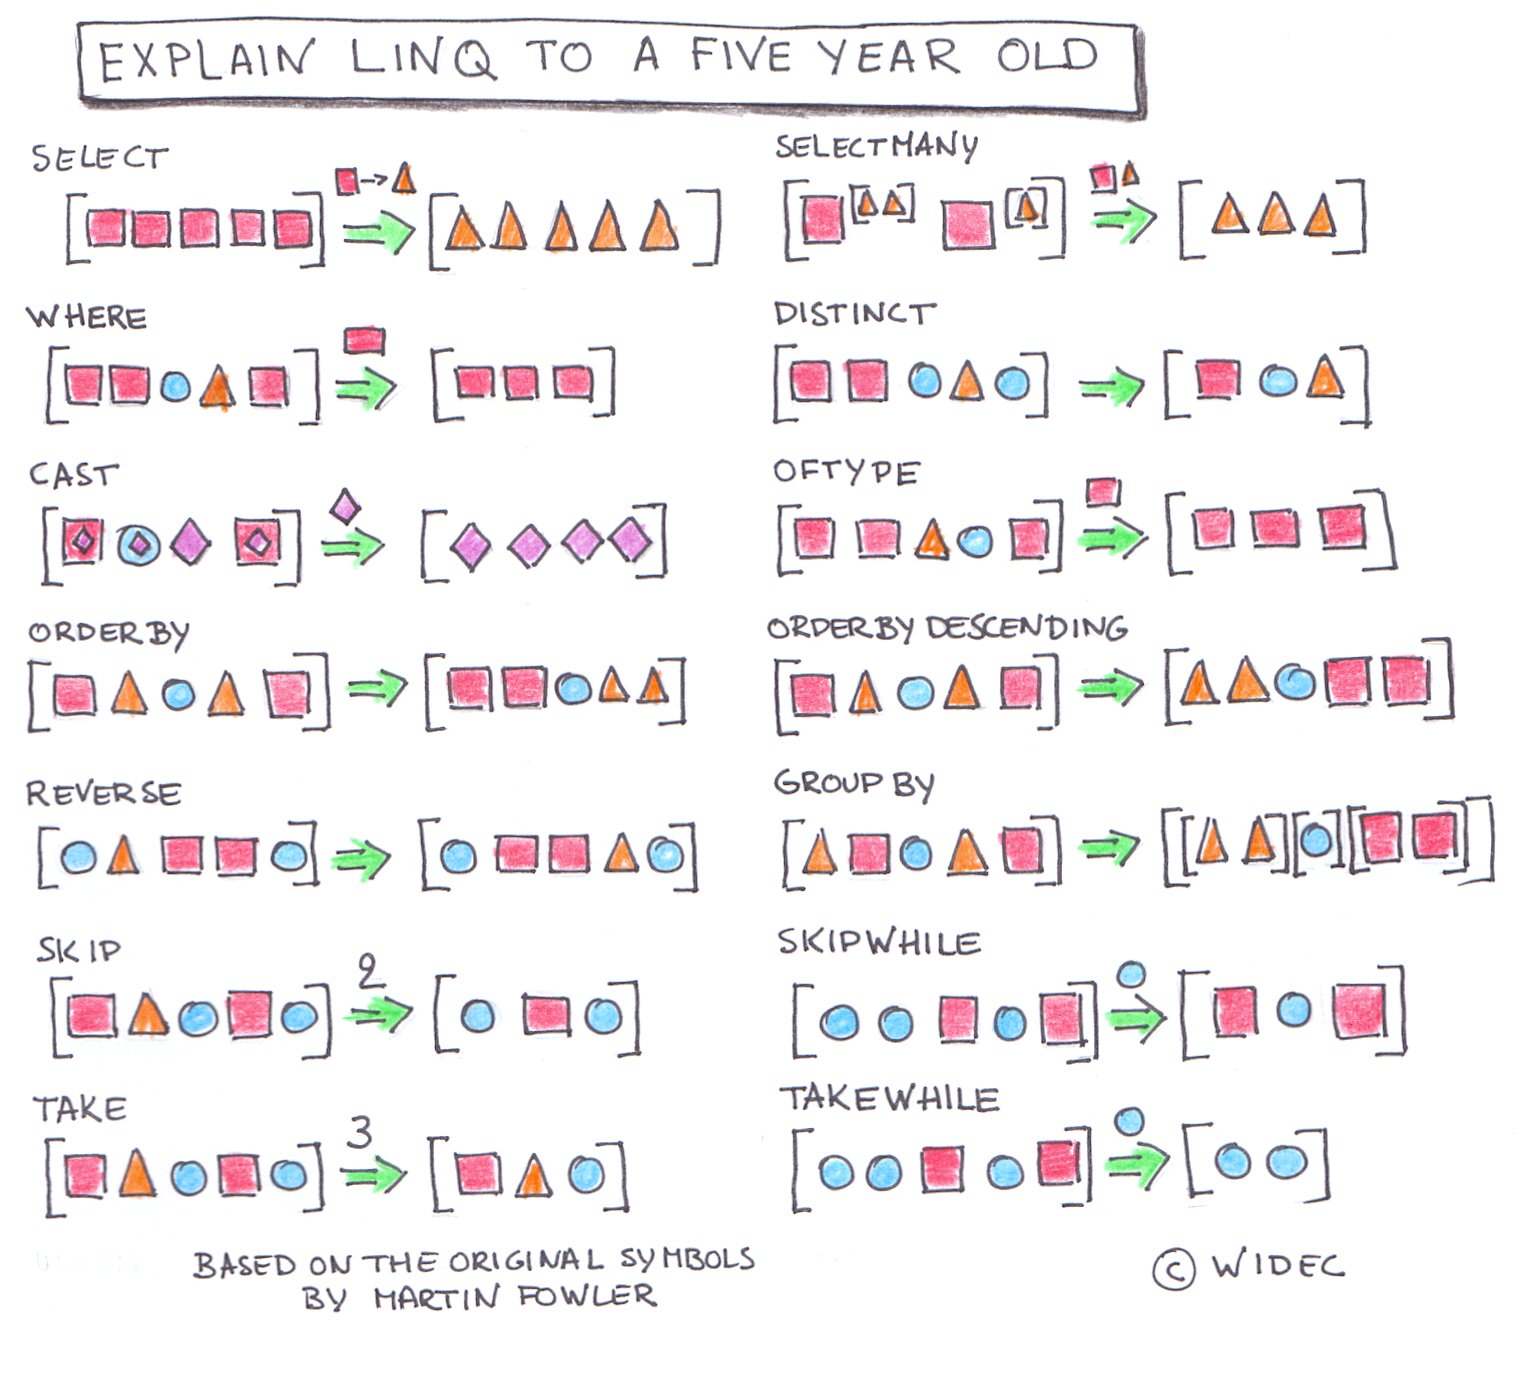
\includegraphics[width=.7\linewidth]{img/linq.jpeg}
  \end{center}

  \tcodeview{2}{8}{20}{\tiny}{\codepath{LinqOperations/Program.cs}}{Example of provisioning operations}

  \tcodeview{2}{22}{49}{\tiny}{\codepath{LinqOperations/Program.cs}}{Example of transformation operations}

  \tcodeview{2}{51}{63}{\tiny}{\codepath{LinqOperations/Program.cs}}{Example of reduction operations}
\end{frame}

\end{document}